\subfigure[Diffusion élastique]{
    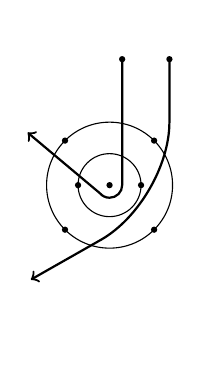
\begin{tikzpicture}[scale=0.4]
        \clip (-2.6, -5) rectangle (2.5, 5);
        \coordinate (O) at (0, 0);
        \coordinate (A) at (0.4, 4);
        \coordinate (B) at (1.9, 4);

        % Circles
        \draw (O) circle (1cm);
        \draw (O) circle (2cm);

        % Central atom
        \fill[black] (O) circle (0.1cm);

        % Atoms on layers # 1
        \fill[black] (0:1) circle (0.1cm);
        \fill[black] (180:1) circle (0.1cm);

        % Atoms on layers # 2
        \fill[black] (45:2) circle (0.1cm);
        \fill[black] (90+45:2) circle (0.1cm);
        \fill[black] (180+45:2) circle (0.1cm);
        \fill[black] (270+45:2) circle (0.1cm);

        % Incident atoms
        \fill[black] (A) circle (0.1cm);
        \fill[black] (B) circle (0.1cm);

        \draw[->, thick ] (A) -- (0.4, 0) arc (0:-140:0.4) -- ++ (140:3);
        \draw[->, thick, rounded corners=1cm ] (B) -- ++(0, -4.5) -- (-2.5, -3);

    \end{tikzpicture}
    \label{fig-chap2-interactions-a}
}\quad
\subfigure[Diffusion inélastique]{\small
    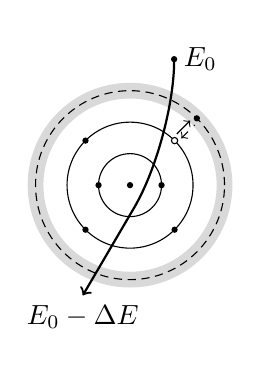
\begin{tikzpicture}[scale=0.4]
        \clip (-3.25, -5) rectangle (3.25, 5);

        \coordinate (O) at (0, 0);
        \coordinate (A) at (1.4, 4);

        % Circles
        \draw (O) circle (1cm);
        \draw (O) circle (2cm);

        % Central atom
        \fill[black] (O) circle (0.1cm);

        % Atoms on layers # 1
        \fill[black] (0:1) circle (0.1cm);
        \fill[black] (180:1) circle (0.1cm);

        % Atoms on layers # 2
        \filldraw [draw=black, fill=white] (45:2) circle (0.1cm);
        \fill[black] (90+45:2) circle (0.1cm);
        \fill[black] (180+45:2) circle (0.1cm);
        \fill[black] (270+45:2) circle (0.1cm);

        % Layer # 3
        \fill [black!15, even odd rule] (O) circle (3.25cm) circle (2.75cm);
        \draw [densely dashed] (O) circle (3cm);

        % Incident atoms
        \fill[black] (A) circle (0.1cm);
        \draw (A) node [right] {$E_0$};
        \draw[->, thick, rounded corners=1cm ] (A) -- ++(0, -2.55) -- (-1.5, -3.5) node [below] {$E_0-\Delta E$};

        % Other atom and arrows
        \fill [black] (45:3) circle (0.1cm);
        \draw [->, rotate=45] (2.2, 0.1) -- ++ (0.6, 0);
        \draw [<-, dashed, rotate=45] (2.2,- 0.1) -- ++ (0.6, 0);

    \end{tikzpicture}
    \label{fig-chap2-interactions-b}
}\quad
\subfigure[Transition énergétique en diffusion inélastique]{\small
    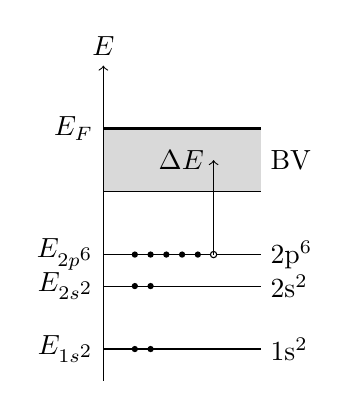
\begin{tikzpicture}[scale=0.4]
        %\clip (-3.25, -4) rectangle (3.25, 4);

        % horiz. lines
        \draw (0, 1) node [left] {$E_{\text{1s\textsuperscript{2}}}$} -- (5, 1) node [right] {1s\textsuperscript{2}};
        \draw (0, 3) node [left] {$E_{\text{2s\textsuperscript{2}}}$} -- (5, 3) node [right] {2s\textsuperscript{2}};
        \draw (0, 4) node [left] {$E_{\text{2p\textsuperscript{6}}}$} -- (5, 4) node [right] {2p\textsuperscript{6}};

        % Valance band
        \fill [black!15] (0, 6) -- (5, 6) -- (5, 8) -- (0, 8) -- cycle;
        \draw (0, 6) -- (5, 6);
        \draw [thick] (0, 8) node [left] {$E_F$} -- (5, 8);
        \draw (5, 7) node [right] {BV};

        % Left axis
        \draw [->] (0, 0) -- (0, 10) node[above] {$E$};

        % Atoms
        \foreach \n in {1, 1.5}{\fill [black] (\n, 1) circle (0.1cm);}
        \foreach \n in {1, 1.5}{\fill [black] (\n, 3) circle (0.1cm);}
        \foreach \n in {1, 1.5, ..., 3}{\fill [black] (\n, 4) circle (0.1cm);}

        % Moved atom
        \fill [draw=black, fill=white] (3.5, 4) circle (0.1cm);
        \draw [->] (3.5, 4) -- (3.5, 7) node [left] {$\Delta E$};

    \end{tikzpicture}
    \label{fig-chap2-interactions-c}
}
